\begin{figure}[t]
  \centering
  %\begin{subfigure}[t]{0.01\linewidth}
  %  \textbf{a.}
  %\end{subfigure}
  \begin{subfigure}[t]{0.32\linewidth}
    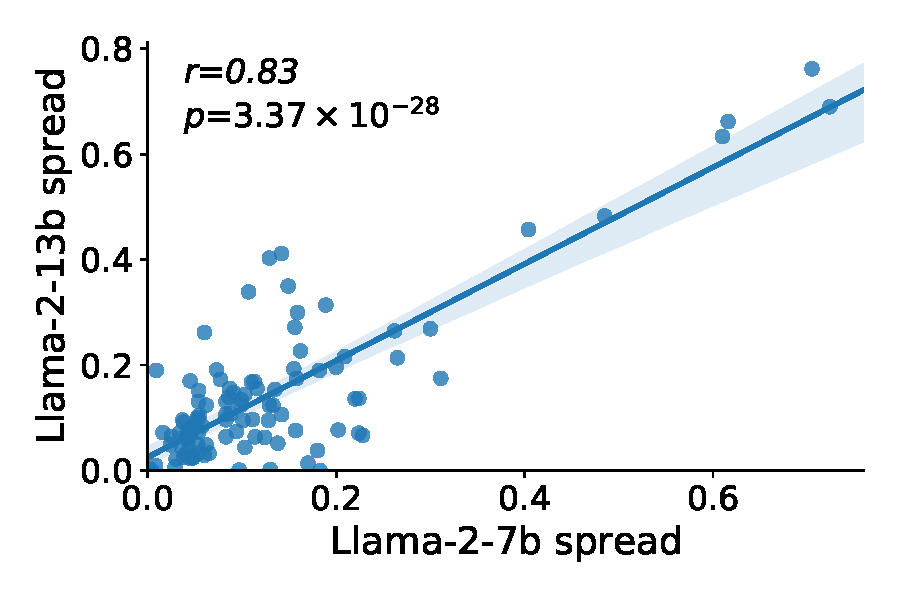
\includegraphics[width=\linewidth, valign=t]{figures/figures_rebuttal/scatter_spread_Llama-2-7b-hf_Llama-2-13b-hf_rankscore_.pdf}
    \vspace{-2mm}
    \caption{Llama-2-7B vs. 13B}\label{fig:perf_spread_llama7b_13b} % perf_spread_llama7b_13b
  \end{subfigure}\hfill
  \begin{subfigure}[t]{0.32\linewidth}
    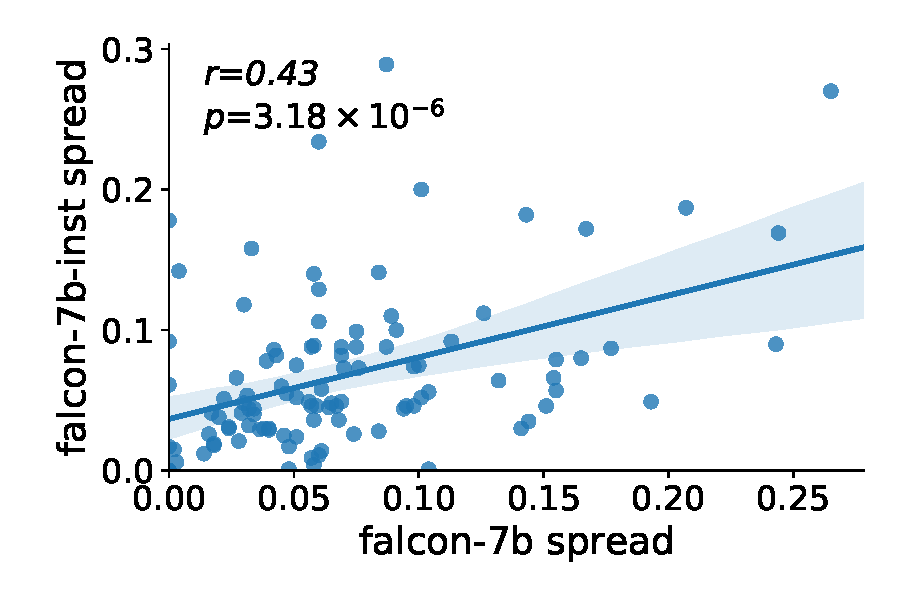
\includegraphics[width=\linewidth, valign=t]{figures/figures_rebuttal/scatter_spread_falcon-7b_falcon-7b-instruct_rankscore_.pdf}
    \vspace{-2mm}\caption{Falcon-7B vs. 7B-Instruct}\label{fig:perf_spread_falcon_7b_inst} % perf_spread_falcon_7b_inst
  \end{subfigure}\hfill
  \begin{subfigure}[t]{0.32\linewidth}
    
\includegraphics[width=\linewidth, valign=t]{figures/figures_rebuttal/scatter_spread_nshot_1_5_rankscore_.pdf}
    \vspace{-2mm}\caption{1-\,vs.\,5-shot\,(same\,task, model)}\label{fig:perf_spread_nshots}  % perf_spread_nshots
  \end{subfigure}\hfill
  \vspace{-1mm}
  \caption{Spread comparison between evaluating the same task under different models or $n$-shots.% \as{we should probably have the x/y axes here the same over all figures, i.e., from 0 to 1, so the visual comparison is easier}\mel{Do you know how to do this in seaborn? I had tried to extend the limits but the shading and interpolation is not extended, so it looks TERRIBLE.}
  % \as{would it be possible to add arrows showing how for particular tasks the performance changes from 1 (blue) to 5 (orange) shot? for the left two figures}\mel{isn't this explicitly covered by the third plot, that shows one spread in x axis and the other in y axis? or do you mean the actual accuracy value?}
  }
\end{figure}

\begin{figure}[t]
\vspace{-3mm}
\begin{minipage}[b]{0.48\linewidth}
    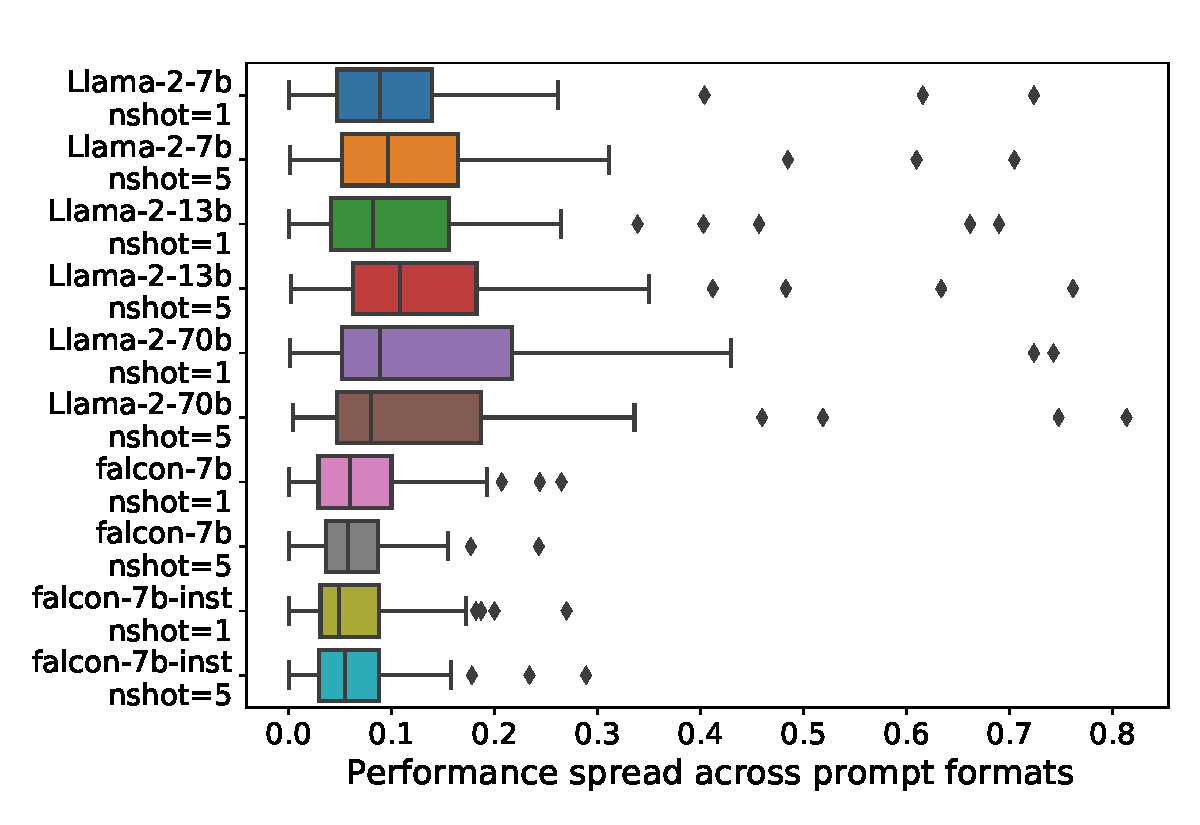
\includegraphics[width=\linewidth, valign=t]{figures/figures_oct_12/boxplot_perf_spread_rankscore_.pdf}
    \vspace{-3mm}\caption{Spread across models and $n$-shots. 
    % \as{this is averaging over all of the tasks we evaluate on?}\mel{the boxplot has one data point per task, yes}
    }\label{fig:perf_spread_boxplot}
\end{minipage}\hfill
\begin{minipage}[b]{0.49\linewidth}
\centering
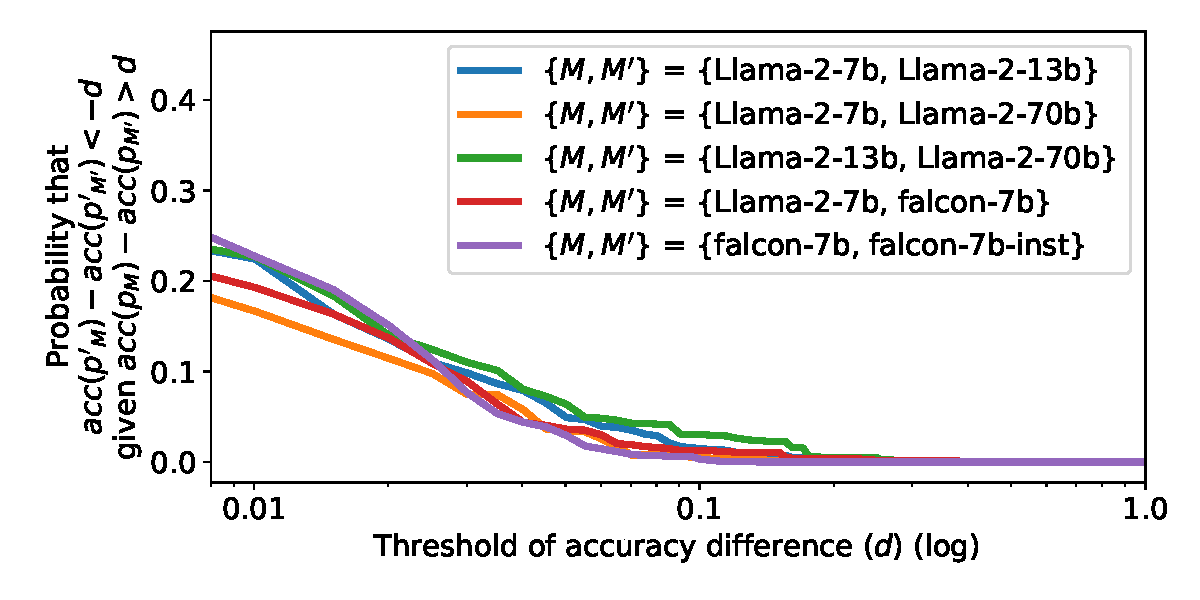
\includegraphics[width=\linewidth, valign=t]{figures/figures_oct_12/probability_of_model_being_better_then_worse_rankscore.pdf}
\vspace{-4mm}\caption{Probability that model $M$ performs \textit{worse} than $M'$ by at least $d$ when using format $p'$, given that $M$ performed \textit{better} than $M'$ by at least $d$  using format $p$. \tbdone{53} tasks, 1- and 5-shot.}\label{fig:model_flip_perf}
    %\caption{\textit{Performance spread across prompt formats.} Metric used is ranking between valid options.}\label{fig:perf_spread}
\end{minipage}
\vspace{-3mm}
\end{figure}
